%----------------------------------------------------------------------------------------------------------------------------------------------------------------------------------
%-------------------------------------------------------------------------------PREAMBLE---------------------------------------------------------------------------------------
%----------------------------------------------------------------------------------------------------------------------------------------------------------------------------------
%
%-------------------Document definition---------------------
\documentclass[compress]{beamer} 
\usepackage{helvet}
\mode<presentation>
%
%---------------------Beamer theme-------------------------
\usetheme{Antibes}{
\usecolortheme{dolphin} % Beamer color theme
}
\useinnertheme{rounded}
\useoutertheme[subsection=false]{miniframes}
\usepackage{etoolbox}
\makeatletter
\patchcmd{\slideentry}{\advance\beamer@tempdim by -.05cm}{\advance\beamer@tempdim by\beamer@vboxoffset\advance\beamer@tempdim by\beamer@boxsize\advance\beamer@tempdim by 1.2\pgflinewidth}{}{}
\patchcmd{\slideentry}{\kern\beamer@tempdim}{\advance\beamer@tempdim by 2pt\advance\beamer@tempdim by\wd\beamer@sectionbox\kern\beamer@tempdim}{}{}
\makeatother
\newcommand*\MyBullet{%
  \item[\color{blue}\scalebox{0.9}{\textbullet}]}
\setbeamertemplate{footline}[frame number]
\setbeamertemplate{navigation symbols}{}
%
%---------------Encoding and other settings-----------------
\usepackage[utf8]{inputenc}
\usepackage[T1]{fontenc}
\usepackage{pgfplots}
\usepackage{tikz}
\usepackage{graphicx}
\definecolor{mygold}{RGB}{255, 153, 0}
\setbeamercolor{item}{bg=mygold,fg=mygold}
\setbeamerfont{section number projected}{%
  family=\rmfamily,series=\bfseries,size=\normalsize}
\setbeamercolor{section number projected}{bg=blue,fg=white}
%
%-----------------------If conditions--------------------------
\newif\ifplacelogo
\placelogotrue % set it to true
\logo{
    \ifplacelogo
    
\includegraphics[keepaspectratio,width=2.5cm]{images/unina}~
    \hspace{\dimexpr\paperwidth-5.5cm-5pt}
    
\includegraphics[keepaspectratio,width=2.8cm]{images/logo_DII}
    \fi
}
\newif\ifplacebackground
\placebackgroundtrue % set it to true
\setbeamertemplate{background canvas}{
    \ifplacebackground
    \rule{0in}{2.6in}%
    \rule{1in}{0in}%
    
\includegraphics[keepaspectratio, width=0.6\paperwidth]{images/unina_vettoriale_con_sigillo.png}
    \fi
}
%
%-----------------------Larger Margin--------------------------
\newcommand\Wider[2][3em]{
\vspace*{-0.8cm}
\makebox[\linewidth][c]{
  \begin{minipage}{\dimexpr\textwidth+#1\relax}
  \raggedright#2
  \end{minipage}
  }
}
%
\newcommand\WiderImages[2][5em]{
\vspace*{-0.5cm}
\makebox[\linewidth][c]{
  \begin{minipage}{\dimexpr\textwidth+#1\relax}
  \raggedright#2
  \end{minipage}
  }
}
%
%-----------------------Title Info--------------------------------
\title{Development of a Java Framework for Parametric Aircraft Design\\
\bigskip
The Performance Analysis Module}
\date{}
%
%----------------------------------------------------------------------------------------------------------------------------------------------------------------------------------
%-------------------------------------------------------------------------------DOCUMENT--------------------------------------------------------------------------------------
%----------------------------------------------------------------------------------------------------------------------------------------------------------------------------------
\begin{document}
%
%-----------------------Title Frame---------------------------
\placelogofalse
\placebackgroundtrue
\begin{frame}
\titlepage
\begin{table}
\begin{tabular}{p{0.7\linewidth}p{0.7\linewidth}}
Relatori: &  Candidato: \\
prof. Fabrizio Nicolosi & Vittorio Trifari \\
prof. Agostino De Marco &  M35/411 \\
\end{tabular}
\end{table}
\end{frame}
%
%--------------------Table of contents-----------------------
\placelogotrue
\placebackgroundfalse
\begin{frame}
\frametitle{Table of Contents}
\tableofcontents
\end{frame}
%
%----------------Current table of contents--------------------
\placelogotrue
\placebackgroundfalse
\begin{frame}{Table of Contents}
\section{Introducing JPAD}
\tableofcontents[currentsection]
\subsection{}
\end{frame}
%
%-----------------------Frame 1-------------------------------
\placelogotrue
\placebackgroundfalse
\begin{frame}{Introducing JPAD - {\Large\textcolor{mygold}{J}}ava {\Large\textcolor{mygold}{P}}rograms for {\Large\textcolor{mygold}{A}}ircraft {\Large\textcolor{mygold}{D}}esign}
\Wider{
\begin{itemize}
\MyBullet A software toolchain for {\textcolor{mygold}{aircraft preliminary design}} and {\textcolor{mygold}{MDO}}
\MyBullet A modern, user friendly, {\textcolor{mygold}{modular framework}}.
\MyBullet Support for {\textcolor{mygold}{simultaneous management/analysis of several aircraft}} and/or ‘varied’ configurations of the same aircraft.
\MyBullet Conceived for {\textcolor{mygold}{collaborative design}} activities.
\MyBullet {\textcolor{mygold}{Interoperability}} with other tools/disciplines (CAD/CFD/FEM analysis).
\end{itemize}
}
\end{frame}
%
%-----------------------Frame 2-------------------------------
\placelogotrue
\placebackgroundfalse
\begin{frame}{Main features}
\Wider{
\begin{itemize}
\MyBullet Define a {\textcolor{mygold}{parametric representations of a complete aircraft}} with XML configuration/input files.
\MyBullet {\textcolor{mygold}{Generate CAD geometries}} of aircraft assembly and sub-components. Measure lengths, areas, volumes. 
\MyBullet {\textcolor{mygold}{Perform various types of analysis}} (L0, L0.5, L1): \textbf{Aerodynamics}, \textbf{Stability \& Control}, \textbf{Performance}, \textbf{Weight \& Balance}, \textbf{Costs}.
\MyBullet Exports {\textcolor{mygold}{analysis results}} in {\textcolor{mygold}{XML}} and {\textcolor{mygold}{Excel formats}}. Produce useful {\textcolor{mygold}{output charts}} for each analysis. 
\MyBullet Perform iterative analysis in order to {\textcolor{mygold}{reach an optimum configuration}}. (\alert{Work in progress}) 
\end{itemize}
}
\end{frame}
%
%-----------------------Frame 3-------------------------------
\placelogotrue
\placebackgroundfalse
\begin{frame}{Java. Why?}
\Wider{
\begin{itemize}
\MyBullet {\textcolor{mygold}{Language widely supported}}. This avoids the library to become obsolete due to the aging of the programming language used.
\MyBullet The language promote the use of {\textcolor{mygold}{open source libraries}}, especially for I/O tasks and for complex mathematical operations.
\MyBullet {\textcolor{mygold}{Widely supported GUI frameworks}} (SWT/JFace and JavaFX) and a GUI visual builders.
\MyBullet {\textcolor{mygold}{Object-Oriented paradigm}} is naturally applied in the abstraction of typical Aircraft Design problems.
\MyBullet Promotes {\textcolor{mygold}{modularity}}: easier to work with in an ever changing team.
\end{itemize}
}
\end{frame}
%
%-----------------------Frame 4-------------------------------
\placelogotrue
\placebackgroundfalse
\begin{frame}{TIOBE Programming Community Index}
\WiderImages{
\begin{figure}[t]
\centering
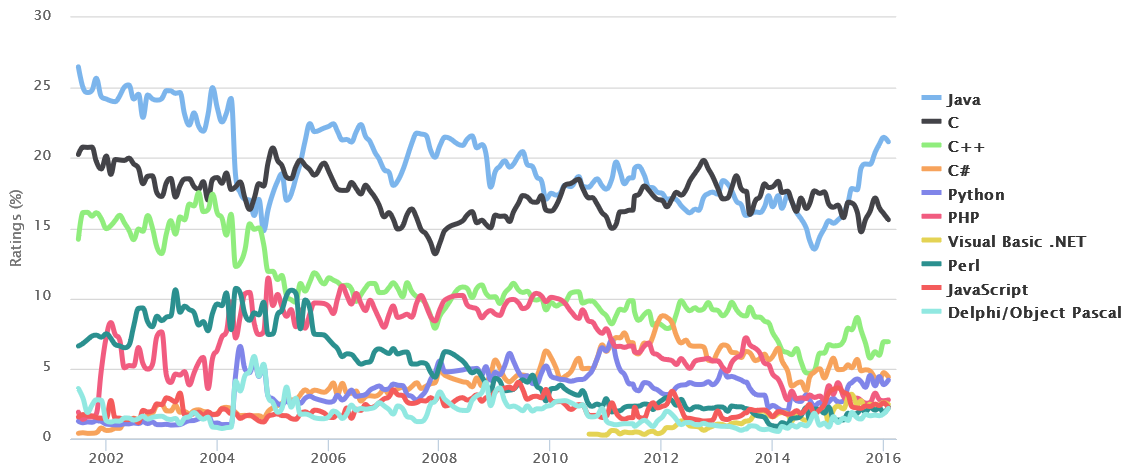
\includegraphics[keepaspectratio, width=\paperwidth]{images/LanguageTrend}
\end{figure}
}
\end{frame}
%
%-----------------------Frame 5-------------------------------
\placelogotrue
\placebackgroundfalse
%
\setbeamertemplate{background canvas}{
    \rule{0in}{3.4in}%
    \rule{0.56in}{0in}%
    \centering
    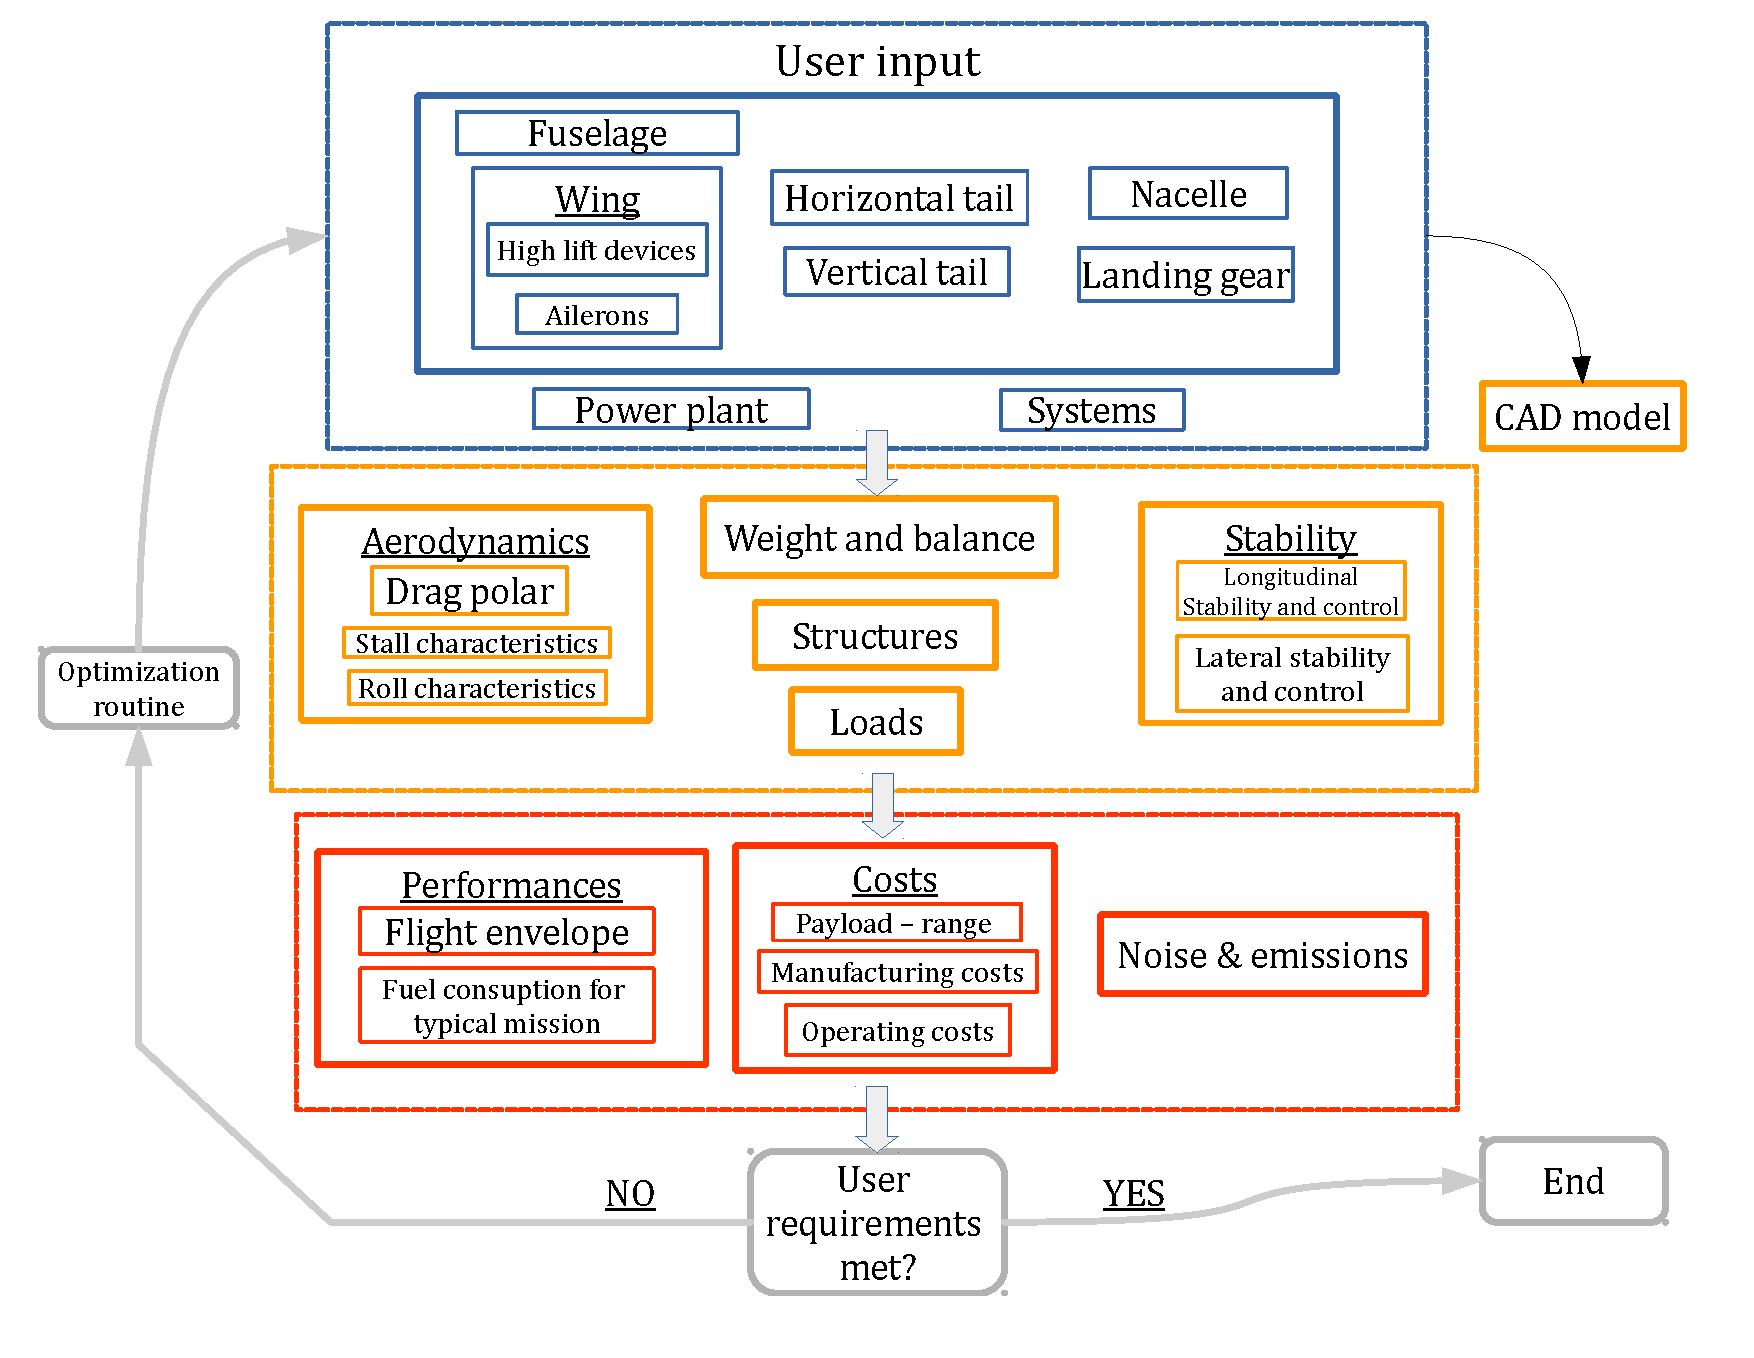
\includegraphics[keepaspectratio, width=0.7\paperwidth]{images/flowchart3}
}
%
\begin{frame}{JPAD typical work session}
\end{frame}
\setbeamertemplate{background canvas}{ }
%
%-----------------------Frame 6-------------------------------
\placelogotrue
\placebackgroundfalse
\begin{frame}{Input file}
\Wider{
The input file type chosen is the {\textcolor{mygold}{XML}} (\emph{{\textcolor{mygold}{eXtensible Markup Language}}}). It is a markup language that defines a set of rules for encoding documents in a format which is both \emph{{\textcolor{mygold}{human-readable}}} and \emph{{\textcolor{mygold}{machine-readable}}}; moreover its design goals of emphasize simplicity, generality and usability across the Internet.
%
\begin{itemize}
\MyBullet \emph{{\textcolor{mygold}{Markup Language}}} due to the use of tags that describes the content.
\MyBullet \emph{{\textcolor{mygold}{extensible}}} because the markup symbols are unlimited and self-defining, so that it is possible to use a personal tag for each data.
\end{itemize}
}
\end{frame}
%
%-----------------------Frame 7-------------------------------
\placelogotrue
\placebackgroundfalse
%
\setbeamertemplate{background canvas}{
    \rule{0in}{3.4in}%
    \rule{0.385in}{0in}%
    \centering
    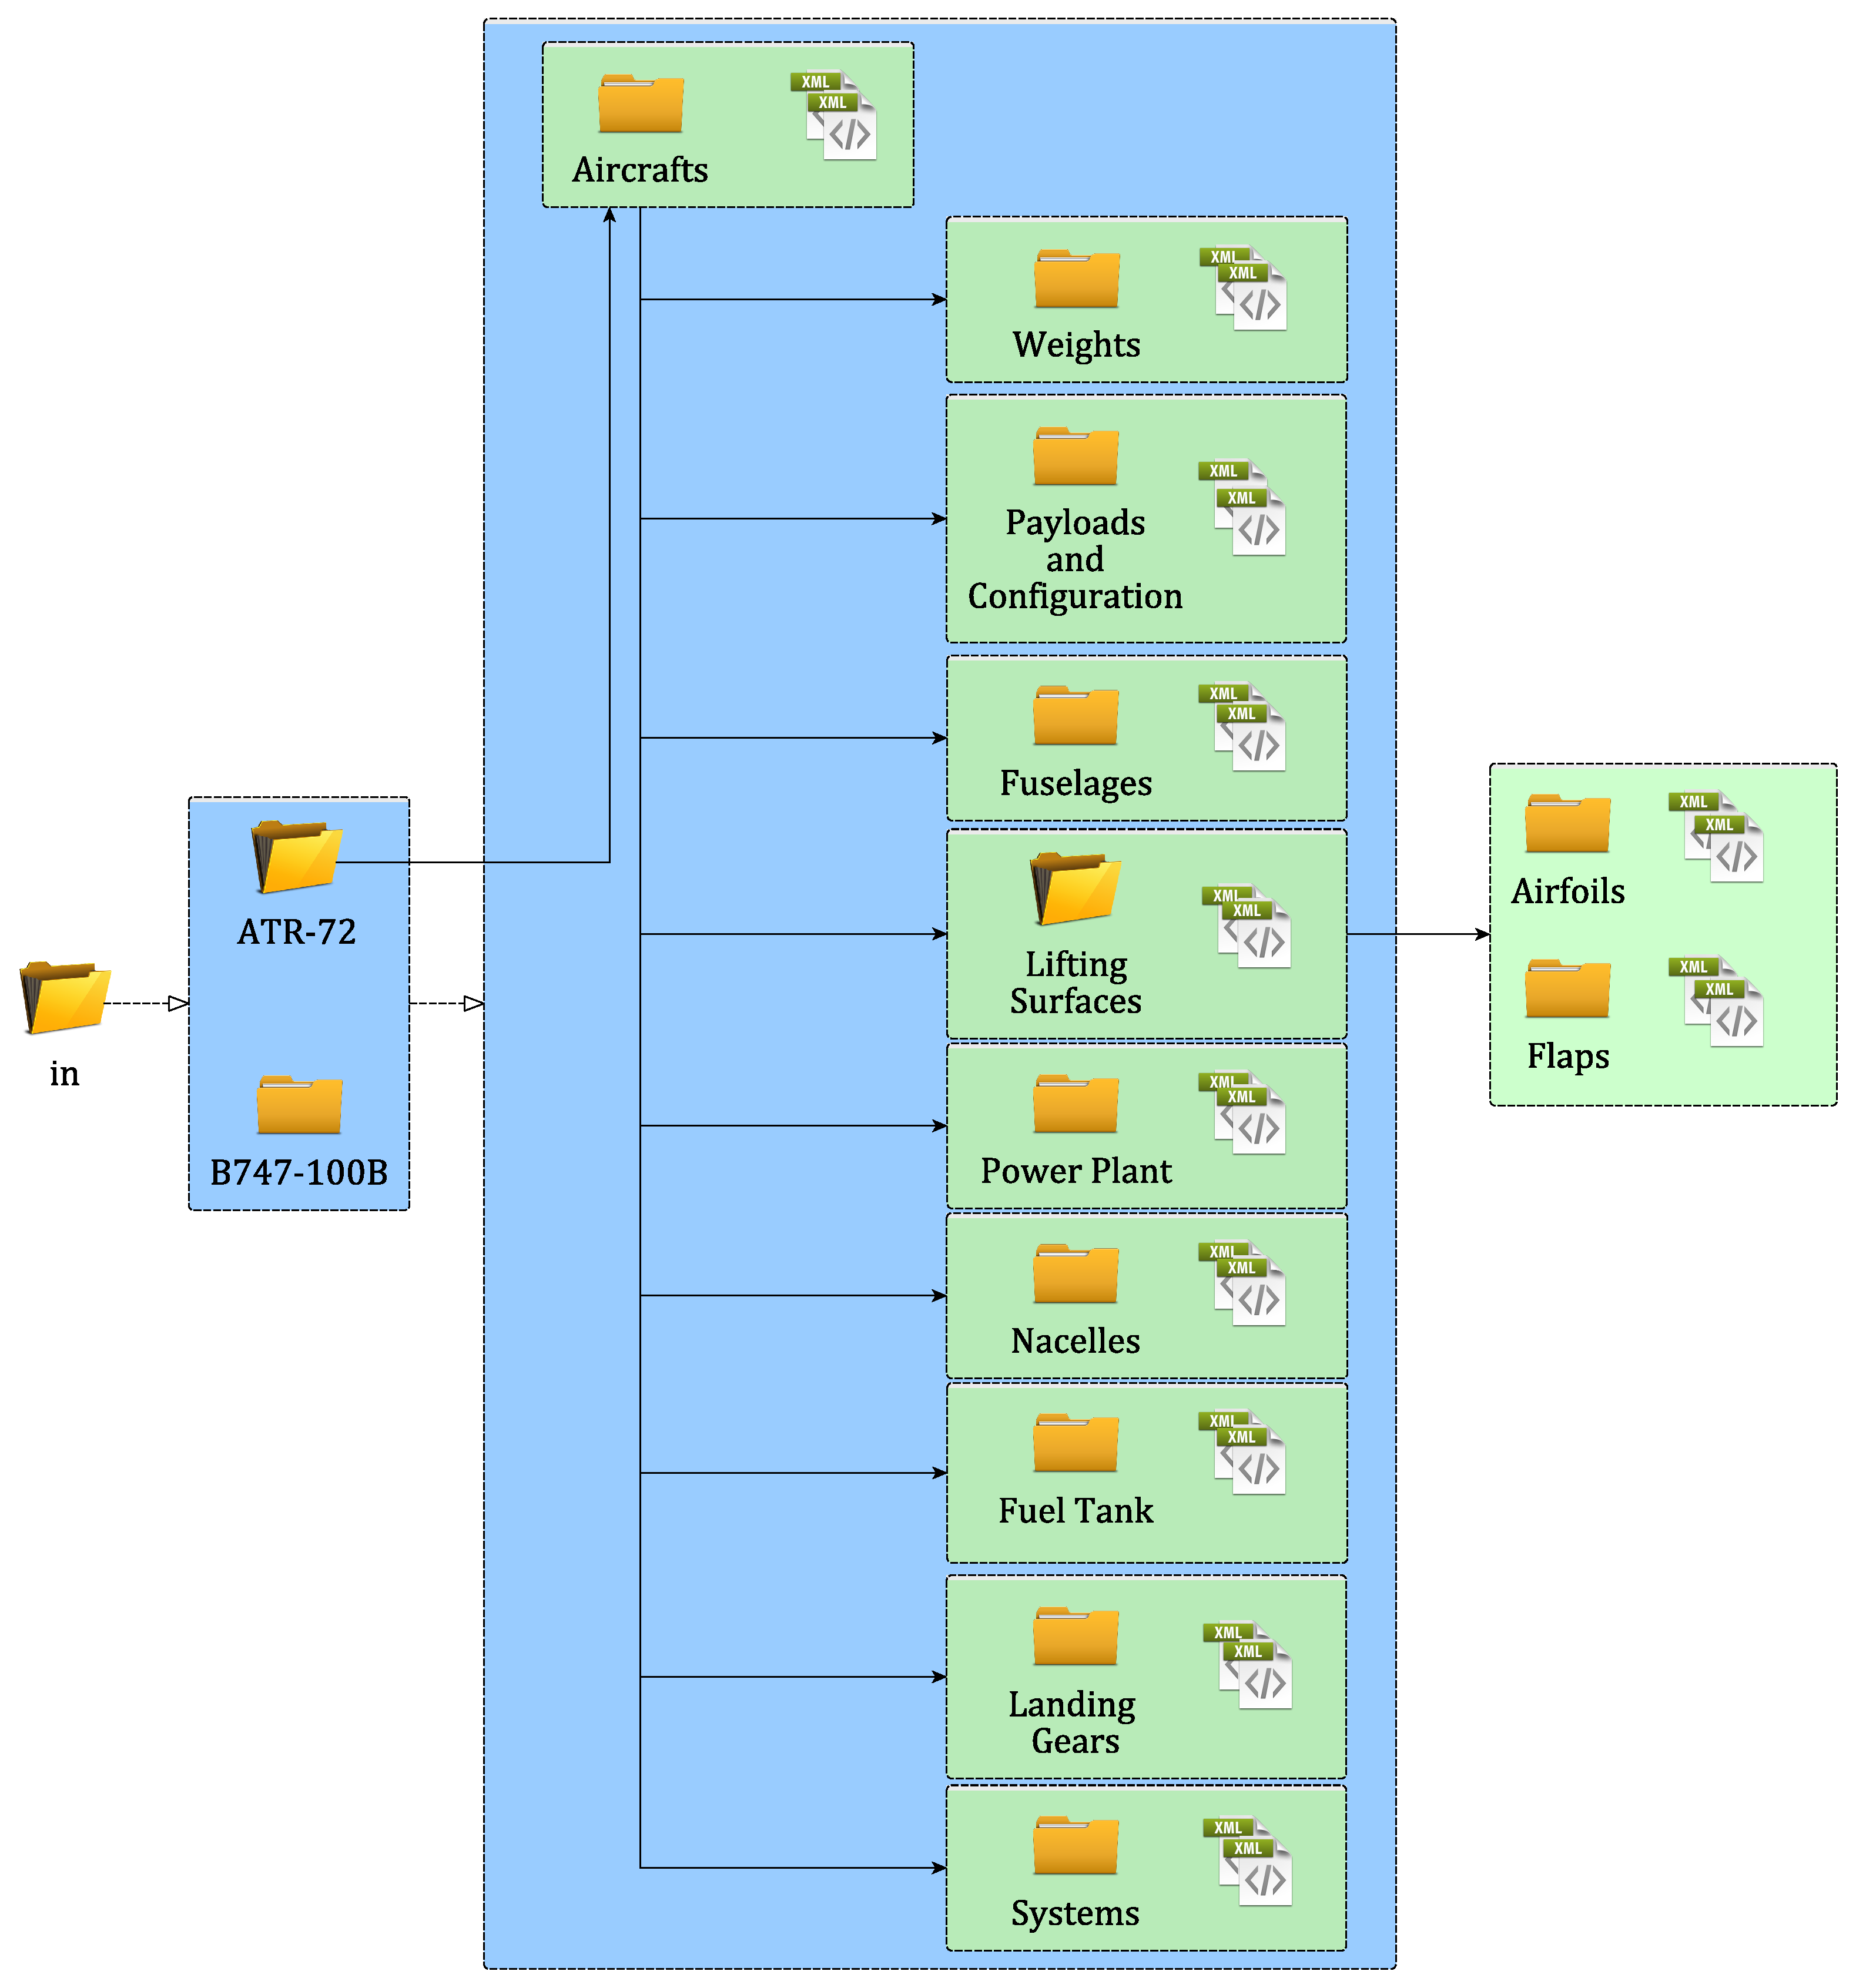
\includegraphics[keepaspectratio, width=0.52\paperwidth]{images/Folder_Tree}
}
%
\begin{frame}{Input file structure prototype}
\begin{figure}[!t]
    \hspace*{6.56cm}
    \vspace*{2cm}
    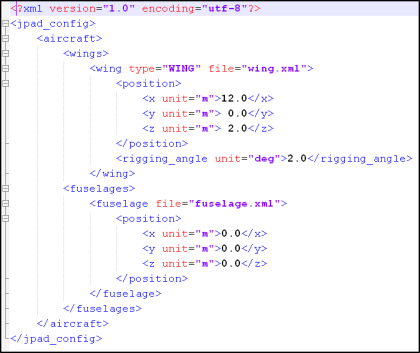
\includegraphics[keepaspectratio, width=0.4\paperwidth]{images/XMLAircraft}
\end{figure}
\end{frame}
\setbeamertemplate{background canvas}{ }
%
%-----------------------Frame 8-------------------------------
\placelogotrue
\placebackgroundfalse
%
\setbeamertemplate{background canvas}{
    \rule{0in}{2.775in}%
    \rule{2in}{0in}%
    \centering
    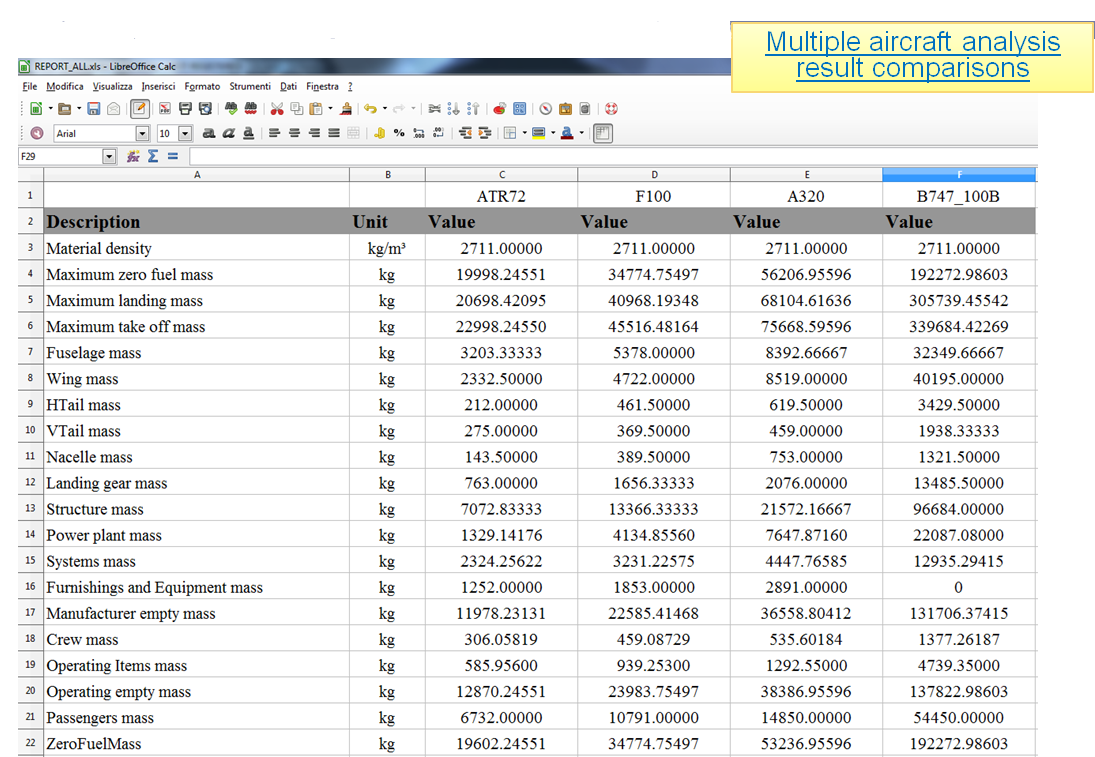
\includegraphics[keepaspectratio, width=0.6\paperwidth]{images/XLS}
}
%
\begin{frame}{JPAD Output}
\Wider{
\begin{itemize}
    \vspace*{-2cm}
\MyBullet XML
\MyBullet Microsoft Excel
\MyBullet Charts
\MyBullet CAD model
\end{itemize}
\begin{figure}[!t]
    \hspace*{-7.7cm}
    \vspace*{-3cm}
    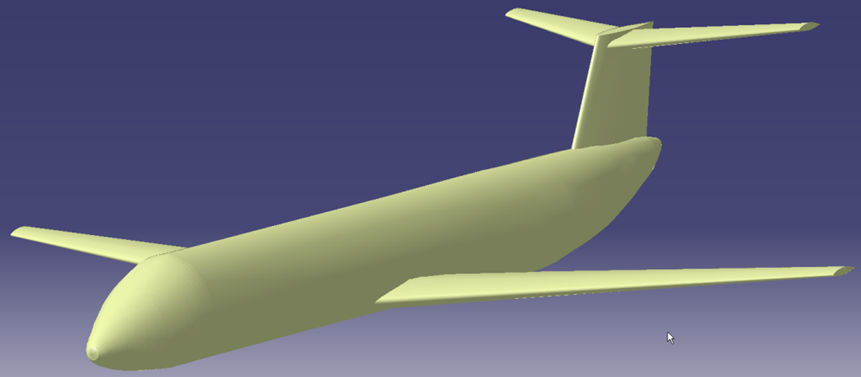
\includegraphics[keepaspectratio, width=0.4\paperwidth]{images/CAD}
\end{figure}
}
\end{frame}
%
\setbeamertemplate{background canvas}{}
%
%-----------------------Frame 9-------------------------------
\placelogotrue
\placebackgroundfalse
\begin{frame}{ADOpT GUI}
\Wider{
\begin{itemize}
	\MyBullet {\textcolor{mygold}{Menu bar}}, holds all the available actions.
	\MyBullet {\textcolor{mygold}{Toolbar}}, holds the actions needed to interact with the application.
	\MyBullet {\textcolor{mygold}{Project tree}}, provides access to all the aircraft components and the analysis results any time.
	\MyBullet {\textcolor{mygold}{3D view}}, shows the CAD model which can be updated each time.
	\MyBullet {\textcolor{mygold}{Log message window}}, tells the status of pending operations.
	\MyBullet {\textcolor{mygold}{Tab folder}}, contains all the windows opened.
\end{itemize}
}
\end{frame}
%
%-----------------------Frame 10-------------------------------
\placelogotrue
\placebackgroundfalse
%
\setbeamertemplate{background canvas}{
    \rule{0in}{3.12in}%
    \rule{0.1in}{0in}%
    \centering
    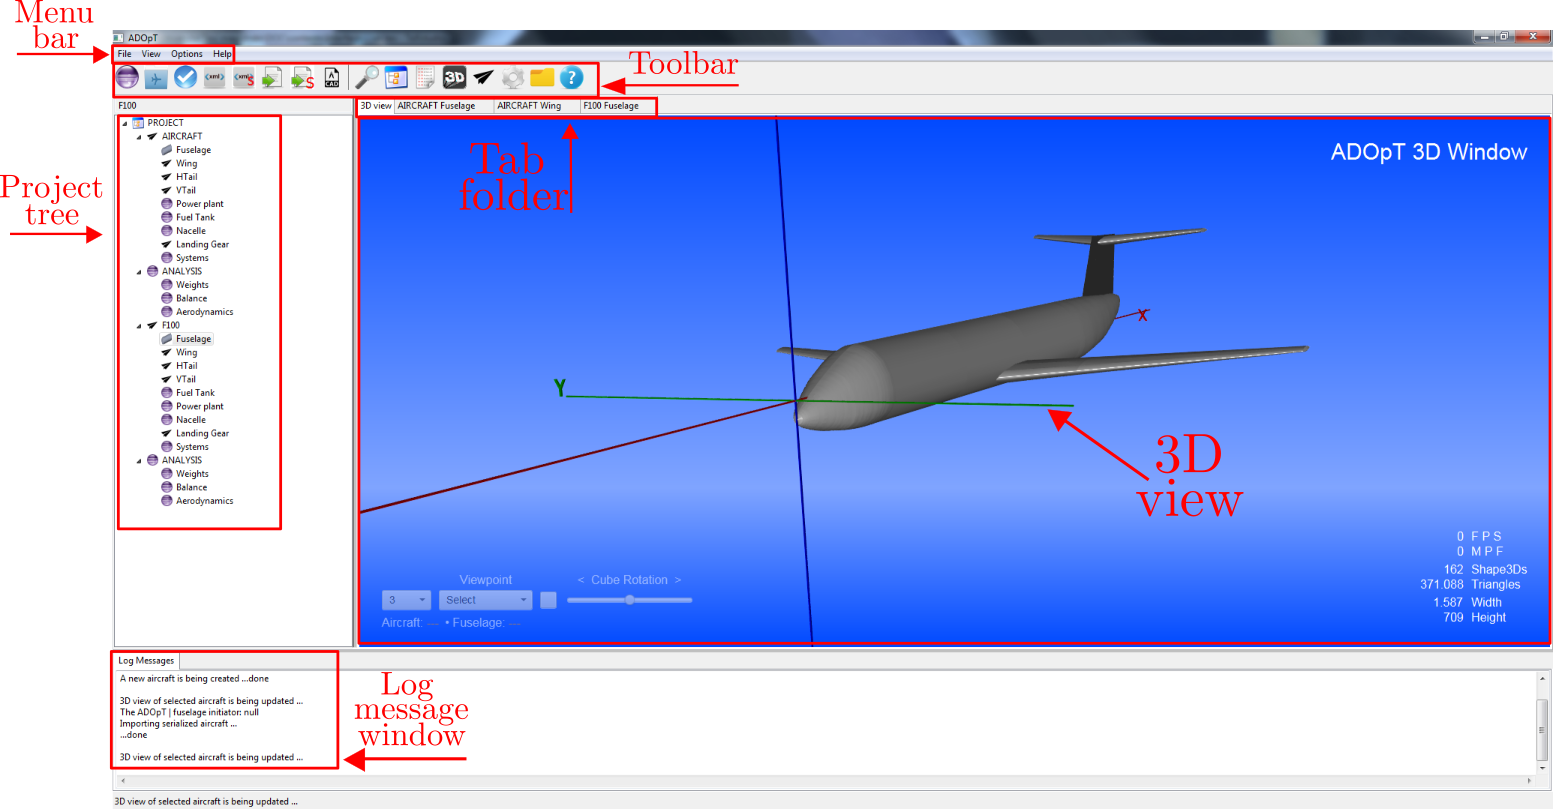
\includegraphics[keepaspectratio, width=0.95\paperwidth]{images/GUI}
}
%
\begin{frame}{ADOpT GUI - Layout}
\end{frame}
\setbeamertemplate{background canvas}{ }
%
%-----------------------Frame 11-------------------------------
\placelogotrue
\placebackgroundfalse
%
\setbeamertemplate{background canvas}{
    \rule{0in}{3.5in}%
    \rule{0.3in}{0in}%
    \centering
    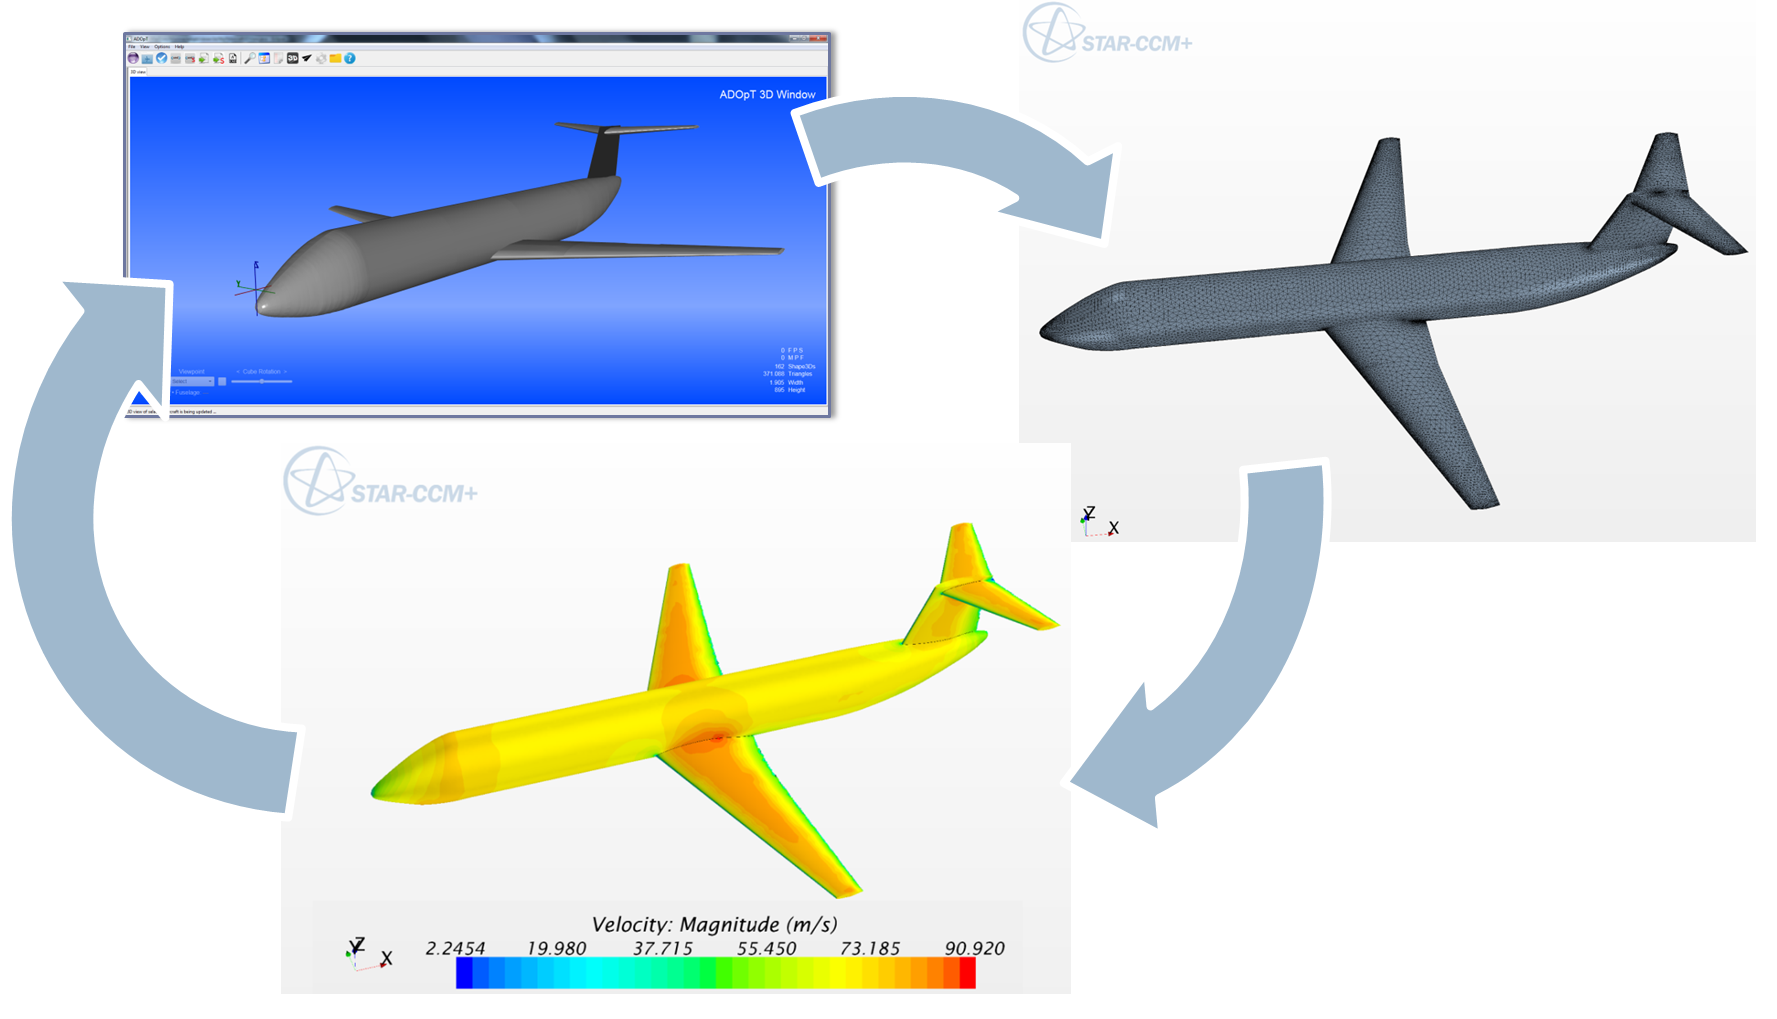
\includegraphics[keepaspectratio, width=0.94\paperwidth]{images/interface}
}
%
\begin{frame}{Interoperability}
\end{frame}
\setbeamertemplate{background canvas}{ }
%
%----------------Current table of contents--------------------
\placelogotrue
\placebackgroundfalse
\begin{frame}{Table of Contents}
\section{The performance analysis module}
\tableofcontents[currentsection]
\subsection{}
\end{frame}
%
%-----------------------Frame 12-------------------------------
\end{document}